\documentclass[openany, amssymb, psamsfonts]{amsart}
\usepackage{mathrsfs,comment}
\usepackage{csquotes}
\MakeOuterQuote{"}
\usepackage[usenames,dvipsnames]{color}
\usepackage[normalem]{ulem}
\usepackage{url}
\usepackage{mhchem}
\usepackage{siunitx}
\usepackage{tikz}
\usetikzlibrary{bending}
\usepackage[all,arc,2cell]{xy}
\UseAllTwocells
\usepackage{enumerate}
%%% hyperref stuff is taken from AGT style file
\usepackage{hyperref}  
\hypersetup{%
    bookmarksnumbered=true,%
    bookmarks=true,%
    colorlinks=true,%
    linkcolor=blue,%
    citecolor=blue,%
    filecolor=blue,%
    menucolor=blue,%
    pagecolor=blue,%
    urlcolor=blue,%
    pdfnewwindow=true,%
    pdfstartview=FitBH}   
  
\let\fullref\autoref
%
%  \autoref is very crude.  It uses counters to distinguish environments
%  so that if say {lemma} uses the {theorem} counter, then autrorefs
%  which should come out Lemma X.Y in fact come out Theorem X.Y.  To
%  correct this give each its own counter eg:
%                 \newtheorem{theorem}{Theorem}[section]
%                 \newtheorem{lemma}{Lemma}[section]
%  and then equate the counters by commands like:
%                 \makeatletter
%                   \let\c@lemma\c@theorem
%                  \makeatother
%
%  To work correctly the environment name must have a corrresponding 
%  \XXXautorefname defined.  The following command does the job:
%
\def\makeautorefname#1#2{\expandafter\def\csname#1autorefname\endcsname{#2}}
%
%  Some standard autorefnames.  If the environment name for an autoref 
%  you need is not listed below, add a similar line to your TeX file:
%  
%\makeautorefname{equation}{Equation}%
\def\equationautorefname~#1\null{(#1)\null}
\makeautorefname{footnote}{footnote}%
\makeautorefname{item}{item}%
\makeautorefname{figure}{Figure}%
\makeautorefname{table}{Table}%
\makeautorefname{part}{Part}%
\makeautorefname{appendix}{Appendix}%
\makeautorefname{chapter}{Chapter}%
\makeautorefname{section}{Section}%
\makeautorefname{subsection}{Section}%
\makeautorefname{subsubsection}{Section}%
\makeautorefname{theorem}{Theorem}%
\makeautorefname{thm}{Theorem}%
\makeautorefname{cor}{Corollary}%
\makeautorefname{lem}{Lemma}%
\makeautorefname{prop}{Proposition}%
\makeautorefname{pro}{Property}
\makeautorefname{conj}{Conjecture}%
\makeautorefname{defn}{Definition}%
\makeautorefname{notn}{Notation}
\makeautorefname{notns}{Notations}
\makeautorefname{rem}{Remark}%
\makeautorefname{quest}{Question}%
\makeautorefname{exmp}{Example}%
\makeautorefname{ax}{Axiom}%
\makeautorefname{claim}{Claim}%
\makeautorefname{ass}{Assumption}%
\makeautorefname{asss}{Assumptions}%
\makeautorefname{con}{Construction}%
\makeautorefname{prob}{Problem}%
\makeautorefname{warn}{Warning}%
\makeautorefname{obs}{Observation}%
\makeautorefname{conv}{Convention}%


%
%                  *** End of hyperref stuff ***

%theoremstyle{plain} --- default
\newtheorem{thm}{Theorem}[section]
\newtheorem{cor}{Corollary}[section]
\newtheorem{prop}{Proposition}[section]
\newtheorem{lem}{Lemma}[section]
\newtheorem{prob}{Problem}[section]
\newtheorem{conj}{Conjecture}[section]
%\newtheorem{ass}{Assumption}[section]
%\newtheorem{asses}{Assumptions}[section]

\theoremstyle{definition}
\newtheorem{defn}{Definition}[section]
\newtheorem{ass}{Assumption}[section]
\newtheorem{asss}{Assumptions}[section]
\newtheorem{ax}{Axiom}[section]
\newtheorem{con}{Construction}[section]
\newtheorem{exmp}{Example}[section]
\newtheorem{notn}{Notation}[section]
\newtheorem{notns}{Notations}[section]
\newtheorem{pro}{Property}[section]
\newtheorem{quest}{Question}[section]
\newtheorem{rem}{Remark}[section]
\newtheorem{warn}{Warning}[section]
\newtheorem{sch}{Scholium}[section]
\newtheorem{obs}{Observation}[section]
\newtheorem{conv}{Convention}[section]

%%%% hack to get fullref working correctly
\makeatletter
\let\c@obs=\c@thm
\let\c@cor=\c@thm
\let\c@prop=\c@thm
\let\c@lem=\c@thm
\let\c@prob=\c@thm
\let\c@con=\c@thm
\let\c@conj=\c@thm
\let\c@defn=\c@thm
\let\c@notn=\c@thm
\let\c@notns=\c@thm
\let\c@exmp=\c@thm
\let\c@ax=\c@thm
\let\c@pro=\c@thm
\let\c@ass=\c@thm
\let\c@warn=\c@thm
\let\c@rem=\c@thm
\let\c@sch=\c@thm
\let\c@equation\c@thm
\numberwithin{equation}{section}
\makeatother

\bibliographystyle{plain}

%--------Meta Data: Fill in your info------
\title{Basic Algebra in Inorganic Chemistry}

\author{Steven Labalme}

\begin{document}




\begin{abstract}
    This paper defines the basics of group theory and representation theory with a focus on domains that are applicable to foundational inorganic chemistry. Subgroups are introduced and Lagrange's theorem proved. Group actions and the relationship of groups and permutations are extended into representation theory. Representations are defined in the abstract and their applicable use in $\mathbb{R}^3$ as representing symmetries recovered as a special case. Lastly, the relationship between all theoretical tenets and the chemistry in which they are used are discussed.
\end{abstract}



\maketitle
\tableofcontents



\section{Introduction}
New advances in mathematics are often driven by the study of worldly phenomena. As such, when chemists realized that important consequences of molecular structure (as defined by the wave equation) are based in molecular symmetry, they needed a rigorous mathematical foundation on which to construct their theory. Moreover, since the wave equation is not solveable in terms of elementary functions, chemists have turned to alternate, more indirect methods of analyzing its properties. Arguably the most common of these is group theory, which is applied through the bridge of representation theory to describe the symmetry of various molecules, the symmetry being directly related to a number of chemical properties. This paper will lay out the basics of group theory and explain how some of its theorems have been applied to chemistry and to what end.



\section{Group Theory}
% \begin{itemize}
%     \item Key ideas in abstract algebra.
%     \begin{itemize}
%         \item Abstract algebra is the study of structure, or more specifically, what a certain structure implies about algebraic objects having that structure.
%         \item The real numbers, which we're quite used to working with, are a continuum and an ordered field, thus satisfying many axioms that imply a rich theory.
%         \item However, studying sets of objects that satisfy far fewer axioms can be equally rewarding, and broadly applicable.
%     \end{itemize}
%     \item A group $\langle G,\cdot\rangle$, for example, is a set $G$ along with a binary operation $\cdot$ on $G$ that satisfies three group axioms, those being that $\cdot$ is associative, that there exists an identity element $e\in G$ satisfying $e\cdot g=g\cdot e=g$ for all $g\in G$, and that for all $g\in G$, there exists an $h\in G$ such that $g\cdot h=h\cdot g=e$.
%     \item Examples of groups:
%     \begin{itemize}
%         \item $\langle\mathbb{Z},+\rangle$ is a group.
%         \item The set $G=\{0,1,2\}$ under addition modulo 3 is a group.
%     \end{itemize}
%     \item One of the first things we can do once we have defined a group is consider "topologizing" it in a sense. Indeed, we can study subsets of an arbitrary group $G$ that have similar properties.
%     \item The most important among the set of subsets of a group $G$ are \textbf{subgroups}, which are nonempty subsets of $G$ that are closed under products (still formed with the original group operation) and inverses.
%     \begin{thm}
%         A subgroup is a group.
%         \begin{proof}
%             Let $H$ be a subgroup of $G$. To prove that $H$ is a group, it will suffice to show that $H$ satisfies the three group axioms.\par\smallskip
%             Axiom 1: Associativity of the elements in the subgroup follows directly from the associativity of the elements in the context of the original group.\par
%             Axiom 2: Let $g\in H$ be arbitrary. Then by closure under inverses, $g^{-1}\in H$. It by closure under products that $gg^{-1}=e\in H$, as desired.\par
%             Axiom 3: Existence of inverses follows from closure under inverses.
%         \end{proof}
%     \end{thm}
%     \begin{itemize}
%         \item As will be discussed in Section 5, subgroups are of critical importance not only in that they lead to many important results in group theory, but in that they come endowed with properties applicable to other fields.
%         \item However, finding subgroups can be difficult --- there are often many subsets to sort through in the power set of $G$. Thus, it will be useful to eliminate some possibilities right off the bat.
%         \item One of the most effective ways of narrowing our search is with Lagrange's theorem, which we shall now work up to.
%         \item \textbf{Left coset} (of $H$ in $G$): The set of all products $ah$, where $H$ is a subgroup of $G$, $a\in G$ is fixed, and $h$ ranges over $H$. \emph{Denoted by} $aH$.
%         \item \textbf{Right coset} (of $H$ in $G$): The set of all products $ha$, where $H$ is a subgroup of $G$, $a\in G$ is fixed, and $h$ ranges over $H$. \emph{Denoted by} $Ha$.
%         \item In this book, we choose to focus on right cosets.
%         \item If $a\in Hb$, then $Ha=Hb$.
%         \begin{proof}
%             Let $x\in Ha$ be arbitrary. Then there exists $h\in H$ such that $x=ha$. Similarly, since $a\in Hb$, there exists $h'\in H$ such that $a=h'b$. Thus, we have that $x=h(h'b)=(hh')b$ by the associative law. But since $H$ is a subgroup of $G$, $hh'\in H$. Therefore, $x\in Hb$, as desired. The proof is symmetric in the other direction.
%         \end{proof}
%         \item Let $G$ be a group and let $H$ be a fixed subgroup of $G$.
%         \begin{thm}
%             The family of all the cosets $Ha$, as $a$ ranges over $G$, is a partition of $G$.
%             \begin{proof}
%                 To prove that the collection of all cosets of $H$ is a partition of $G$, it will suffice to show that any two cosets are either disjoint or equal, and every element of $G$ is in some coset. We take this one constraint at a time.\par
%                 Let $Ha,Hb$ be arbitrary cosets of $H$ in $G$. We divide into two cases ($Ha,Hb$ are disjoint and $Ha,Hb$ are not disjoint). If they are disjoint, we are done. On the other hand, if they are not disjoint, then there exists $x\in Ha\cap Hb$. Since $x\in Ha$, $x=h_1a$ for some $h_1\in H$. Similarly, $x=h_2b$ for some $h_2\in H$. It follows that $a=(h_1^{-1}h_2)b$. But since $h_1^{-1}h_2\in H$ by the definition of a subgroup, the above fact implies that $Ha=Hb$, as desired.\par
%                 Let $x\in G$ be arbitrary. Since $e\in H$ by the definition of a subgroup, $x=ex\in Hx$, as desired.
%             \end{proof}
%         \end{thm}
%         \item Let $G$ be a finite group, let $H$ be be a fixed subgroup of $G$, and let $a\in G$ be arbitrary.
%         \begin{thm}
%             If $Ha$ is any coset of $H$, there is a one-to-one correspondence from $H$ to $Ha$.
%             \begin{proof}
%                 Let $f:H\to Ha$ be defined by $f(h)=ha$ for all $h\in H$. To prove that $f$ is bijective, it will suffice to show that it is injective and surjective. To begin, let $f(h_1)=f(h_2)$. Then $h_1a=h_2a$. But by the cancellation law, $h_1=h_2$, as desired. Now let $x\in Ha$ be arbitrary. By the definition of $Ha$, $x=ha$ for some $h\in H$. Therefore, $f(h)=ha=x$, as desired.
%             \end{proof}
%         \end{thm}
%         \begin{itemize}
%             \item This implies that if $G$ is finite, all cosets of $H$ have the same number of elements.
%         \end{itemize}
%         \item Let $G$ be a finite group, and $H$ any subgroup of $G$.
%         \begin{thm}[Lagrange's Theorem]
%             The order of $G$ is a multiple of the order of $H$.
%             \begin{proof}
%                 By Theorem 13.1, we may let the cosets of $H$ divide $G$ into $n$ partitions. By Theorem 2, each of these $n$ partitions has the same cardinality $|H|$. Therefore, since the elements in the group are divided into $n$ partitions of size $|H|$, $|G|=n|H|$, as desired.
%             \end{proof}
%         \end{thm}
%         \item Let $G$ be a group.
%         \begin{thm}
%             If $G$ has a prime number $p$ of elements, then $G$ is a cyclic group. Furthermore, any element $a\neq e$ in $G$ is a generator of $G$.
%             \begin{proof}
%                 Let $a$ be an arbitrary non-neutral element of $G$. As we know, $\langle a\rangle$ is a subgroup of $G$. Thus, by Lagrange's theorem, $|\langle a\rangle|\mid|G|$. However, since $|G|=p$ is prime, either $|\langle a\rangle|=1$ or $|\langle a\rangle|=p$. But since $a\neq e$, $|\langle a\rangle|\neq 1$. Therefore, $|\langle a\rangle|=p$, and we have that $G$ is a cyclic group with generator $a$, as desired.
%             \end{proof}
%         \end{thm}
%         \item Theorem 13.4 gives us complete information on all groups of prime order; in other words, every group of prime order is isomorphic to the well-behaved $\mathbb{Z}/p\mathbb{Z}$.
%         \item Let $G$ be a finite group and $a\in G$.
%         \begin{thm}
%             The order of $a$ divides the order of $G$.
%             \begin{proof}
%                 Clearly, $|a|=|\langle a\rangle|$. But since $\langle a\rangle$ is a subgroup of $G$, Lagrange's theorem implies that $|\langle a\rangle|=|a|\mid|G|$, as desired.
%             \end{proof}
%         \end{thm}
%     \end{itemize}
% \end{itemize}

Abstract algebra is the study of the structure of algebraic objects. One of the first examples we become familiar with is the real numbers, which are a continuum and an ordered field, thus satisfying many axioms that imply a rich theory. However, algebra also studies sets of objects that satisfy far fewer axioms.\par
\begin{defn}
    A \textbf{group} $\langle G,\cdot\rangle$ is a set $G$ along with a binary operation $\cdot$ on $G$ that satisfies three group axioms: $\cdot$ is associative, there exists an identity element $e\in G$ satisfying $e\cdot g=g\cdot e=g$ for all $g\in G$, and for all $g\in G$, there exists an $h\in G$ such that $g\cdot h=h\cdot g=e$.
\end{defn}
A simple example of a group is $\langle\mathbb{Z},+\rangle$, or the integers under addition. Addition combines any two integers into a third integer, adding is associative, 0 serves as an additive identity, and the inverse of any integer is its opposite ($-x$ corresponding to $x$).
\begin{defn}
    Let $A$ be a set, and let $[n]$ denote the set of all natural numbers from 1 to $n$, inclusive. If $A$ and $[n]$ are in bijective correspondence, then we say that the \textbf{cardinality} of $A$ is $n$, and denote this by $|A|=n$.
\end{defn}
\begin{defn}
    Let $A$ be a set. If $|A|=n$ where $n\in\mathbb{N}$, then we say that $A$ is \textbf{finite}. If $|A|\neq n$ for any $n\in\mathbb{N}$, then we say that $A$ is \textbf{infinite}.
\end{defn}
Since $\mathbb{Z}$ contains all of the natural numbers and more, $\mathbb{Z}$ is infinite. More rigorously, if we suppose for the sake of contradiction that there exists a bijective correspondence between $\mathbb{Z}$ and $[n]$ for any $[n]$, we can prove that the function is not bijective. Relating this back to group theory, since $\mathbb{Z}$ is infinite, we call a group such as $\langle\mathbb{Z},+\rangle$ an \textbf{infinite group}.\par
Naturally, there also exist \textbf{finite groups}. One of the most well-studied classes of finite groups is the following.
\begin{defn}
    For any $n\in\mathbb{N}$, let $\mathbb{Z}/n\mathbb{Z}$ denote the group defined by the set $\{0,1,2,\dots,n\}$ under addition modulo $n$.
\end{defn}
For example, the set $\mathbb{Z}/2\mathbb{Z}=\{0,1,2\}$ under addition modulo 2 is a finite group. Addition modulo 2 guarantees closure, associativity still holds, 0 is an identity, and inverses are as follows: $-0=0$, $-1=2$, and $-2=1$.\par
Now that we have defined groups, one of the first things we can do is ask about their structure. Indeed, we can study subsets of an arbitrary group $G$ that have similar properties. The most important of the subsets of a group $G$ is defined as follows.
\begin{defn}
    A \textbf{subgroup} $H$ of a group $G$ is a nonempty subset of $G$ that is closed under products (which are still formed with the original group operation) and inverses.
\end{defn}
The first important property of subgroups that we shall prove is the following.
\begin{rem}
    A subgroup is a group.
    \begin{proof}[Justification]
        Let $H$ be a subgroup of $G$. To prove that $H$ is a group, it will suffice to show that $H$ satisfies the three group axioms.\par\smallskip
        Axiom 1: Associativity of the elements in the subgroup follows directly from the associativity of the elements in the context of the original group.\par
        Axiom 2: Let $g\in H$ be arbitrary. Then by closure under inverses, $g^{-1}\in H$. It by closure under products that $gg^{-1}=e\in H$, as desired.\par
        Axiom 3: Existence of inverses follows from closure under inverses.
    \end{proof}
\end{rem}
A simple example of a subgroup is that the \textbf{alternating group} $A_n$ is a subgroup of the \textbf{symmetric group} $S_n$.
\begin{defn}
    Consider the set $[n]$. The \textbf{symmetric group} (of order $n$) is the set of all bijections $f:[n]\to[n]$ under the operation of function composition. \emph{Denoted by} $S_n$.
\end{defn}
In other words, the symmetric group is the set of all permutations of the numbers 1 through $n$. Now, every permutation of an amount of numbers can be written as the product of some number of \textbf{transpositions}, and it can be proven that no permutation can be written as the product of an even number of transpositions \emph{and} an odd number of transpositions. This fact allows for the following definition.
\begin{defn}
    Consider the symmetric group of order $n$. The \textbf{alternating group} (or order $n$) is the subset of $S_n$ consisting of all \emph{even} permutations of order $n$ under the operation of function composition. \emph{Denoted by} $A_n$.
\end{defn}
These definitions allow us to prove the following proposition.
\begin{prop}
    The alternating group $A_n$ is a subgroup of $S_n$.
    \begin{proof}
        To prove that $A_n$ is a subgroup of $S_n$, it will suffice to show that $A_n$ is closed under products and inverses. Let $\sigma,\sigma'\in A_n$ be two even permutations. Then they can be expressed as the product of an even number of transpositions. It follows since the sum of two even numbers is another even number that their product is the product of an even number of transpositions, itself. As to closure under inverses, since the inverse of the transposition $(x\ y)$ is the transposition $(y\ x)$, the inverse of any even permutation is equal to the product of the inverses of each underlying transposition, given in reverse order (e.g., the inverse of $(1\ 2)(3\ 4)$ is $(4\ 3)(2\ 1)$), and thus the product of an even number of transpositions, itself.
    \end{proof}
\end{prop}
As will be discussed in Section 5, subgroups are of critical importance not only in that they lead to many important results in group theory, but in that they come endowed with properties applicable to other fields. However, finding subgroups can be difficult --- there are often many subsets of $G$ to sort through.
\begin{defn}
    Let $G$ be a set. The \textbf{power set} (of $G$) is the set of all subsets of $G$. \emph{Denoted by} $\wp(G)$.
\end{defn}
If $G$ is an infinite group, the power set of $G$ is also infinite (and, in fact, it can be proven that the power set of an infinite group is a of a higher order infinity than that of the original group). If $G$ is a finite group with $|G|=n$, it can be proven that $|\wp(G)|=2^n$. Thus, it will be useful to eliminate some possibilities right off the bat. One of the most effective ways of narrowing our search is with Lagrange's theorem, which we shall now work up to.\par
\begin{defn}
    Let $H$ be a subgroup of $G$. We define each \textbf{right coset} (of $H$ in $G$) to be the set of all products $ha$, where $a\in G$ is fixed and $h$ ranges over the elements of $H$. \emph{Denoted by} $Ha$. Symbolically, we have that
    \begin{equation*}
        Ha = \{ha\mid h\in H\}
    \end{equation*}
\end{defn}
We may analogously define the left coset of $H$ in $G$, but without the loss of generality, we will work with right cosets (all subsequent proofs are naturally symmetric for left cosets).\par
A useful first property of cosets is the following.
\begin{thm}
    If $a\in Hb$, then $Ha=Hb$.
    \begin{proof}
        Let $x\in Ha$ be arbitrary. Then there exists $h\in H$ such that $x=ha$. Similarly, since $a\in Hb$, there exists $h'\in H$ such that $a=h'b$. Thus, we have that $x=h(h'b)=(hh')b$ by the associative law. But since $H$ is a subgroup of $G$, $hh'\in H$. Therefore, $x\in Hb$, as desired. The proof is symmetric in the other direction.
    \end{proof}
\end{thm}
With this result in hand, we are now ready to prove the following.
\begin{thm}
    Let $G$ be a group and let $H$ be a fixed subgroup of $G$. Then the family of all the cosets $Ha$, as $a$ ranges over $G$, is a partition of $G$.
    \begin{proof}
        To prove that the collection of all cosets of $H$ is a partition of $G$, it will suffice to show that any two cosets are either disjoint or equal, and every element of $G$ is in some coset. We take this one constraint at a time.\par
        Let $Ha,Hb$ be arbitrary cosets of $H$ in $G$. We divide into two cases ($Ha,Hb$ are disjoint and $Ha,Hb$ are not disjoint). If they are disjoint, we are done. On the other hand, if they are not disjoint, then there exists $x\in Ha\cap Hb$. Since $x\in Ha$, $x=h_1a$ for some $h_1\in H$. Similarly, $x=h_2b$ for some $h_2\in H$. It follows that $a=(h_1^{-1}h_2)b$. But since $h_1^{-1}h_2\in H$ by the definition of a subgroup, the above fact implies that $Ha=Hb$, as desired.\par
        Let $x\in G$ be arbitrary. Since $e\in H$ by the definition of a subgroup, $x=ex\in Hx$, as desired.
    \end{proof}
\end{thm}
Additionally, we need the following.
\begin{thm}
    Let $G$ be a finite group, let $H$ be be a fixed subgroup of $G$, and let $a\in G$ be arbitrary. If $Ha$ is any coset of $H$, there is a one-to-one correspondence from $H$ to $Ha$.
    \begin{proof}
        Let $f:H\to Ha$ be defined by $f(h)=ha$ for all $h\in H$. To prove that $f$ is bijective, it will suffice to show that it is injective and surjective. To begin, let $f(h_1)=f(h_2)$. Then $h_1a=h_2a$. But by the cancellation law, $h_1=h_2$, as desired. Now let $x\in Ha$ be arbitrary. By the definition of $Ha$, $x=ha$ for some $h\in H$. Therefore, $f(h)=ha=x$, as desired.
    \end{proof}
\end{thm}
We can now combine the last two results in an interesting manner --- we now know that the collection of all cosets of a certain subgroup $H$ partitions $G$ into subsets all of equal cardinality. Thus, \emph{the cardinality of $G$ is a multiple of the cardinality of $H$}. Lagrange's theorem formalizes this notion.
\begin{thm}[Lagrange's Theorem]
    Let $G$ be a finite group, and $H$ any subgroup of $G$. The order of $G$ is a multiple of the order of $H$.
    \begin{proof}
        By Theorem 2.2, we may let the cosets of $H$ divide $G$ into $n$ partitions. By Theorem 2.3, each of these $n$ partitions has the same cardinality $|H|$. Therefore, since the elements in the group are divided into $n$ partitions of size $|H|$, $|G|=n|H|$, as desired.
    \end{proof}
\end{thm}\par
Although a simple result, Lagrange's theorem gives usa  powerful tool in our quest to assert order on groups. One of the most immediate and most striking consequences of Lagrange's theorem is that it completely characterizes all groups of prime order.
\begin{thm}
    Let $G$ be a group. If $G$ has a prime number $p$ of elements, then $G$ is a cyclic group. Furthermore, any element $a\neq e$ in $G$ is a generator of $G$.
    \begin{proof}
        Let $a$ be an arbitrary non-neutral element of $G$. As we know, $\langle a\rangle$ is a subgroup of $G$. Thus, by Lagrange's theorem, $|\langle a\rangle|\mid|G|$. However, since $|G|=p$ is prime, either $|\langle a\rangle|=1$ or $|\langle a\rangle|=p$. But since $a\neq e$, $|\langle a\rangle|\neq 1$. Therefore, $|\langle a\rangle|=p$, and we have that $G$ is a cyclic group with generator $a$, as desired.
    \end{proof}
\end{thm}
Similarly, Lagrange's theorem characterizes all cyclic subgroups of $G$, giving us valuable information about the possible orders of elements in $G$.
\begin{thm}
    Let $G$ be a finite group and $a\in G$. The order of $a$ divides the order of $G$.
    \begin{proof}
        Clearly, $|a|=|\langle a\rangle|$. But since $\langle a\rangle$ is a subgroup of $G$, Lagrange's theorem implies that $|\langle a\rangle|=|a|\mid|G|$, as desired.
    \end{proof}
\end{thm}



\section{Group Actions}
% \begin{itemize}
%     \item A \textbf{group action} is a function $\cdot:G\times A\to A$ satisfying two properties, namely that $g_1\cdot(g_2\cdot a)=(g_1g_2)\cdot a$ for all $g_1,g_2\in G$ and $a\in A$, and that $e\cdot a=a$ for all $a\in A$.
%     \item This is a highly unintuitive definition, so let's see what sense we can make of it.
%     \begin{itemize}
%         \item First off, by the definition of the domain and codomain of $\cdot$, we can see that for an arbitrary $g\in G$, $g$ maps every $a\in A$ to a unique $g\cdot a\in A$.
%         \item Indeed, taking the perspective that each $g\in G$ acts like a function on $A$ will be advantageous.
%         \item However, by property 1, $\cdot$ also makes the effect of $g_1g_2$ on $a$ equivalent to applying $g_2$ first, and then $g_1$ to the resultant product $g_2\cdot a$.
%         \item In other words, the $\cdot$ operation essentially doubles as relating an argument and a function to an output, \emph{and} function composition.
%         \item The second stipulation just guarantees that the identity element of $G$ behaves like an identity function, so that when we "compose" an element $g\in G$ with $e$, the effect of $g$ on $A$ is unaltered, as it should be.
%     \end{itemize}
%     \item Since each $g\in G$ becomes an automorphism of $A$ under the group action definition, a natural use of group actions is to describe permutation functions.
%     \begin{itemize}
%         \item Let $A=\{1,2,3\}$ and $G=\{e,g_1\}$, where
%         \begin{align*}
%             g_1\cdot 1 &= 1&
%             g_1\cdot 2 &= 3&
%             g_1\cdot 3 &= 2
%         \end{align*}
%         and
%         \begin{center}
%             \begin{tabular}{r|cc}
%                       & $e$   & $g_1$\\
%                 \hline
%                 $e$   & $e$   & $g_1$\\
%                 $g_1$ & $g_1$ & $e$\\
%             \end{tabular}
%         \end{center}
%         is the group multiplication table.
%         \item It is trivial, albeit tedious, to show that the group action $\cdot$ satisfies properties 1-2 as defined, so the explicit proof will be omitted.
%         \item Although it may have seemed to be an unnecessary formalism at first, the usefulness of group actions should now be more clear. Indeed, group actions allow us to rigorously abstract the group-like properties of permutation functions and apply all of the results of group theory to them.
%     \end{itemize}
% \end{itemize}

\begin{defn}
    A \textbf{group action} is a function
    \begin{equation*}
        (\ \cdot\ ):G\times A\to A
    \end{equation*}
    satisfying two properties, namely that $g_1\cdot(g_2\cdot a)=(g_1g_2)\cdot a$ for all $g_1,g_2\in G$ and $a\in A$, and that $e\cdot a=a$ for all $a\in A$.
\end{defn}
By the definition of the domain and codomain of $\cdot$, we can see that for an arbitrary $g\in G$, $g$ maps every $a\in A$ to a unique $g\cdot a\in A$. Indeed, each $g\in G$ acts like a function on $A$. However, by property 1, $\cdot$ also makes the action of $g_1g_2$ on $a$ equivalent to applying $g_2$ first, and then $g_1$ to the resultant product $g_2\cdot a$ (this is associativity). In other words, the $\cdot$ operation essentially doubles as relating an argument and a function to an output, \emph{and} function composition. The second stipulation just guarantees that the identity element of $G$ behaves like an identity function, so that when we "compose" an element $g\in G$ with $e$, the effect of $g$ on $A$ is unaltered, as it should be.\par
Since each $g\in G$ becomes an automorphism of $A$ under the group action definition, a natural use of group actions is to describe permutations. For example, let $A=\{1,2,3\}$ and $S_2=\{e,g\}$, where
\begin{align*}
    g\cdot 1 &= 1&
    g\cdot 2 &= 3&
    g\cdot 3 &= 2
\end{align*}
and
\begin{center}
    \begin{tabular}{r|cc}
            & $e$ & $g$\\
        \hline
        $e$ & $e$ & $g$\\
        $g$ & $g$ & $e$\\
    \end{tabular}
\end{center}
is the group multiplication table. It is trivial, albeit tedious, to show that the group action $\cdot$ satisfies properties 1-2 as defined, so the explicit proof will be omitted. Indeed, group actions allow us to rigorously abstract the group-like properties of permutation functions and apply all of the results of group theory to them.



\section{Linear Representations}
% \begin{itemize}
%     % \item One of the more important sets of objects that obey group-like properties are symmetry operations. Although we usually think of symmetry through the lens of planes and axes of symmetry, it is equivalent to consider the \emph{action of reflecting/rotating the object about said planes and axes}. Since any two symmetry operations performed consecutively will still be \emph{some} kind of symmetry operation, albeit perhaps not a traditionally intuitive one, the operation of function composition on the set of symmetry operations guarantees closure. The other axioms can be shown to hold as well. It is this group-like character of symmetry operations of a given figure under function composition that motivates representation theory.
%     % \item Think about a
%     \item Informally, a representation maps each element in a group to an automorphism of a vector space onto itself in an order-preserving manner, where group multiplication becomes function composition. Let's now build up to this formally.
%     \item Let $V$ be an $n$-dimensional vector space over the complex numbers. We define the \textbf{general linear group of degree \emph{n}} to be the set of all linear mappings from $V$ to $V$. We denote this group by $GL_n(\mathbb{C})$.
%     \item It follows that there is a one-to-one correspondence between $GL_n(\mathbb{C})$ and the set of $n$-square invertible matrices.
%     \item If we let $G$ be a finite group, then $\rho:G\to GL_n(\mathbb{C})$ is a \textbf{representation} of $G$ if and only if $\rho$ is a homomorphism.
%     \item Essentially, $\rho$ renames linear transformations with the elements of $G$ so that we can study how they combine in the abstract, and assert back the structure that our group theory provides upon linear transformations. In the other direction, representation theory brings to bear the powerful tools of abstract linear algebra upon group theory, and provides a method for visualizing how group elements interact.
%     \item Alright, well now that we have vastly expanded group theory into $\mathbb{C}^n$, things get more complicated. For instance, two representations may be essentially the same, but encapsulated by entirely different matrices since in $n$-space, coordinate systems are relative. Thus, we need to define when two representations are similar, and in fact, we do so in the same way we do in linear algebra. Indeed, two representations $\rho$ and $\rho'$ are similar if there exists a linear transformation $\tau$ such that $\rho(s)=\tau\circ\rho'(s)\circ\tau^{-1}$ for all $s\in G$.
%     \item Now that we can equate similar representations across differing coordinate systems, we might ask what the simplest coordinate system is that we can use. This question motivates the introduction of the \textbf{regular representation}. Let $(e_t)_{t\in G}$ be a standard basis indexed by the elements of $G$. Then we can quite simply let each $\rho(s)$ be the permutation matrix that sends $e_t\mapsto e_{st}$. This representation will be very easy to work with, and we can equate it with many others through similarity.
%     \item It is also worth noting that technically, we can let $\rho:G\to GL_n(\mathbb{C})$ be defined by $\rho(s)=e$ for all $s\in G$, where $e$ is the identity function on $\mathbb{C}$. However, this will obviously yield little information about anything, and we mention it only for the sake of mathematical completeness. This representation is referred to as the \textbf{trivial representation}.
%     \item A curious thing to note is that in finite groups, every element has finite order. In other words, for any $s\in G$, $s^n=e$ for some $n\in\mathbb{N}$. This necessitates a curious constraint on the representation of an arbitrary finite group $G$.
%     \begin{thm}
%         If $R_s$ is the $n$-square invertible matrix associated with $\rho(s)$, then $\det(R_s)$ is a root of unity.
%         \begin{proof}
%             Since $s^n=e$, $R_s^n=E$. Thus, $|R_S|^n=1$, so $|A|=\sqrt[n]{1}$.
%         \end{proof}
%     \end{thm}
% \end{itemize}

Representation theory was originally motivated by the desire to study groups and other algebraic objects by what they act on. Group actions formalize the notion of a group acting on a set, and representation theory takes the next step of formalizing the notion of a group acting on a vector space, a well-studied and well-defined mathematical object that can provide great reverse insight into algebraic structure.\par
Informally, a representation maps each element in a group to an automorphism of a vector space onto itself in an order-preserving manner, where group multiplication becomes function composition. Let's now build up to this formally.
\begin{defn}
    Let $V$ be an $n$-dimensional vector space over the complex numbers. We define the \textbf{general linear group of degree \emph{n}} to be the set of invertible linear mappings from $V$ to $V$. \emph{Denoted by} $GL_n(\mathbb{C})$. Symbolically, we have that
    \begin{equation*}
        GL_n(\mathbb{C}) = \{f:V\to V\mid f\text{ is linear \& invertible}\}
    \end{equation*}
\end{defn}
It follows that there is a one-to-one correspondence between $GL_n(\mathbb{C})$ and the set of $n$-square invertible matrices. We are now ready to define a representation of a finite group.
\begin{defn}
    Let $G$ be a finite group. Then a \textbf{linear representation} (of $G$) is a homomorphism $\rho:G\to GL_n(\mathbb{C})$.
\end{defn}
Note that since two representations may be essentially the same, but be encapsulated by entirely different matrices since in $n$-space, coordinate systems are relative.
\begin{defn}
    Two representations $\rho$ and $\rho'$ are \textbf{similar} if there exists a linear transformation $\tau$ such that $\rho(s)=\tau\circ\rho'(s)\circ\tau^{-1}$ for all $s\in G$.
\end{defn}
In the same way that we can use conjugation to convert between bases in linear algebra, conjugation allows us to convert between the bases of the matrices in the general linear group, matching up representations that are the same in different coordinate systems.\par
Now that we can equate similar representations across differing coordinate systems, we might ask what the simplest coordinate system is that we can use. This question motivates the following definition.
\begin{defn}
    Let $(e_t)_{t\in G}$ be a standard basis indexed by the elements of $G$. Then the \textbf{regular representation} (of $G$) equates each $\rho(s)$ with the permutation matrix that sends $e_t\mapsto e_{st}$.
\end{defn}
This representation will be very easy to work with, and we can equate it with many others through similarity.\par
In the same realm of simple representations, it is also worth mentioning the following.
\begin{defn}
    The \textbf{trivial representation} is the representation $\rho:G\to GL_n(\mathbb{C})$ defined by $\rho(s)=e$ for all $s\in G$, where $e$ is the identity function on $\mathbb{C}$.
\end{defn}
As an example, consider the group $C_{2v}=\{e,C_2,\sigma_v,\sigma_v'\}$ with a group operation defined by
\begin{center}
    \begin{tabular}{c|cccc}
                    & $e$         & $C_2$       & $\sigma_v$  & $\sigma_v'$\\
        \hline
        $e$         & $e$         & $C_2$       & $\sigma_v$  & $\sigma_v'$\\
        $C_2$       & $C_2$       & $e$         & $\sigma_v'$ & $\sigma_v$ \\
        $\sigma_v$  & $\sigma_v$  & $\sigma_v'$ & $e$         & $C_2$      \\
        $\sigma_v'$ & $\sigma_v'$ & $\sigma_v$  & $C_2$       & $e$        \\
    \end{tabular}
\end{center}
One example of a representation of this group is the homomorphism $\rho:C_{2v}\to GL_3(\mathbb{C})$ defined by
\begin{align*}
    \rho(e) &=
    \begin{bmatrix}
        1 & 0 & 0\\
        0 & 1 & 0\\
        0 & 0 & 1\\
    \end{bmatrix}&
        \rho(C_2) &=
        \begin{bmatrix}
            -1 & 0 & 0\\
            0 & -1 & 0\\
            0 & 0 & 1\\
        \end{bmatrix}\\
    \rho(\sigma_v) &=
    \begin{bmatrix}
        1 & 0 & 0\\
        0 & -1 & 0\\
        0 & 0 & 1\\
    \end{bmatrix}&
        \rho(\sigma_v') &=
        \begin{bmatrix}
            -1 & 0 & 0\\
            0 & 1 & 0\\
            0 & 0 & 1\\
        \end{bmatrix}
\end{align*}
It can be checked that the representation as defined is a homomorphism.\par
A curious thing to note is that in finite groups, every element has finite order. In other words, for any $s\in G$, $s^n=e$ for some $n\in\mathbb{N}$. This necessitates a constraint on the representation of an arbitrary finite group $G$.
\begin{thm}
    If $R_s$ is the $n$-square invertible matrix associated with $\rho(s)$, then $\det(R_s)$ is a root of unity.
    \begin{proof}
        Since $s^n=e$, $R_s^n=E$. Thus, $|R_S|^n=1$, so $|A|=\sqrt[n]{1}$.
    \end{proof}
\end{thm}



\section{Connections to Chemistry}
% \begin{itemize}
%     \item What do we notice about symmetry operations on a given molecule, specifically in the realm of composing them with each other? We notice that the composition of any two symmetry operations is another symmetry operation. We notice that there is an identity symmetry operation. We notice that composition is associative. And we notice that the inverse of any symmetry operation is also a symmetry operation. Now sometimes, there might be special properties: For example, commutativity holds for the set of symmetry operations applicable to \ce{H2O}, but not to the set applicable to \ce{NH3}. However, the four properties listed first (closure, identity, associativity, and inverse) \emph{always} hold. Here is where we abstract. We define a group to be set of objects along with an operation for combining them that satisfies these four axioms. Indeed, based off of just this simple description, there is a rich field of observations we can make about such algebraic structures, that can then in turn be applied back to chemistry. Here, we will discuss some of the more significantly applicable results of group theory and how representation theory formally applies them back to physical reality.
%     \item In IChem, molecules of point group G often share properties with molecules of point group H, where H is a subgroup of G. Finding subgroups can be tricky though, so we need tools to make our search easier. The most powerful of these tools is Lagrange's theorem.
% \end{itemize}

Motivated by the need to understand the vibrational modes of molecules, which are heavily dependent on their symmetry, inorganic chemists took the budding field of representation theory and applied it to their work. The connection is actually quite simple. Representation theory essentially abstracts the group-like character of automorphisms of a vector space, and a symmetry operation can be thought of as an automorphism of $\mathbb{R}^3$, specifically one that maps a certain set of points onto itself, permuting them linearly. All of these factors --- automorphisms, linear transformations, and permutations --- dramatically evoke representation theory, and indeed it has been a valuable tool for pulling information out of the algebraically unsolveable wave equation.\par
As chemists have refined their understanding of reaction kinetics over the years, they have gone from "two molecules must meet at the right speed and with the correct orientation in order to react" to "two orbitals must be within 10 electron volts of each other and have the same symmetry in order to form a molecular orbital." Thus, symmetry point groups, the foundation of molecular symmetry, directly govern which molecules can react, how they react, and to what extent, all without having to directly solve the wave equation for many many electrons and nuclei.\par
\begin{center}
    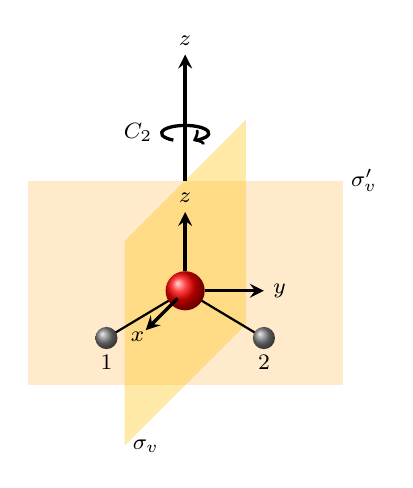
\begin{tikzpicture}
        \footnotesize
        \fill [orange!80!yellow,opacity=0.2] (-2,-1.2) rectangle (2,1.4) node[black,opacity=1,right]{$\sigma_v'$};
        \fill [orange!50!yellow,opacity=0.35] (0,-1.2,-2) -- (0,1.4,-2) -- (0,1.4,2) -- (0,-1.2,2) node[black,opacity=1,right]{$\sigma_v$};
        \draw [very thick,-stealth] (0,1.4,0) -- (0,3,0) node[above]{$z$};
        \draw [yshift=2cm,very thick,arrows={->[scale width=0.6,flex=2]}] (-120:0.3cm and 0.1cm) arc[start angle=240,end angle=-70,x radius=0.3cm,y radius=0.1cm] node[xshift=-7mm,yshift=1mm]{$C_2$};

        \draw [thick] (-1,-0.6) node[circle,ball color=gray]{} node[below=1mm]{1} -- (0,0) node[circle,ball color=red,inner sep=5pt]{} -- (1,-0.6) node[circle,ball color=gray]{} node[below=1mm]{2};

        \draw [very thick,-stealth] (0.25,0,0) -- (1,0,0) node[right]{$y$};
        \draw [very thick,-stealth] (0,0.25,0) -- (0,1,0) node[above]{$z$};
        \draw [very thick,-stealth] (0,0,0.25) -- (0,0,1.3) node[below left=-1mm]{$x$};
    \end{tikzpicture}
\end{center}
The group $C_{2v}$ discussed above is an example of a symmetry point group. In fact, it is the symmetry point group that describes the \ce{H2O} molecule, pictured above. Indeed, each group element can be thought of a symmetry operation, with $e$ keeping the molecule where it is, $C_2$ rotating the molecule by $\frac{\ang{360}}{2}=\ang{180}$ about the $z$-axis, $\sigma_v$ reflecting the molecule across the $xz$-plane, and $\sigma_v'$ reflecting the molecule across the $yz$-plane. This property of the elements of $C_{2v}$ is best captured by the given representation, which consists of linear automorphisms that directly describe each symmetry element: $\rho(\sigma_v)$, for example, is a matrix describing the reflection of a vector over the $xz$-plane, just like the symmetry operation in the picture above.\par
Besides mapping structure to properties, more advanced realms of group theory are also applicable to inorganic chemistry. For example, the now familiar domain of subgroups plays an important role in governing the properties of molecules with very complex point groups. For the linear molecule \ce{CO2}, for instance, the presence of an infinite rotation axis means that the group multiplication table corresponding to \ce{CO2} is quite unwieldy and computationally intensive to do anything with. However, there is a simple finite subgroup of this infinite group (namely $D_{2h}$) that captures well enough the important vibrational modes of \ce{CO2} in a much less computationally intensive manner. Similarly, Lagrange's theorem allows us to easily determine the possible subgroups of any molecule, and thus compare its vibrational modes with those of molecules corresponding solely to its subgroups.



\section*{Acknowledgments}
It is a pleasure to thank my mentor, Micah Gay, for pointing me to books that would begin my journey into the realm of algebra. I would also like to thank Danny Espejo for recommending \cite{pinter}, specifically, an accessible yet rigorous introduction group theory that clarified a great deal of the motivation and fundamental concepts of Abstract Algebra.



\begin{thebibliography}{9}
    \bibitem{pinter}
    Charles C. Pinter.
    A Book of Abstract Algebra.
    Dover. 2010.

    \bibitem{DummitFoote}
    David S. Dummit and Richard M. Foote.
    Abstract Algebra.
    John Wiley and Sons. 2004.
    
    \bibitem{Serre}
    Jean-Paul Serre.
    Linear Representations of Finite Groups.
    Springer. 1971.
\end{thebibliography}




\end{document}